% Welcome! This is the unofficial University of Udine beamer template.

% See README.md for more informations about this template.

% This style has been developed following the "Manuale di Stile"
% (Style Manual) of the University of Udine. You can find the
% manual here: https://www.uniud.it/it/ateneo-uniud/ateneo-uniud/identita-visiva/manuali-immagine-stile/manuale-stile

% Note: for some reason, the RGB values specified in the manual
% do NOT render correctly in Beamer, so they have been redefined
% for this document using the high level chromo-optic deep neural 
% quantistic technology offered by Microsoft Paint's color picker.

% We defined four theme colors: UniBrown, UniBlue, UniGold
% and UniOrange. For example, to write some uniud-brownish
% text, just use: \textcolor{UniBrown}{Hello!}

% Note that [usenames,dvipsnames] is MANDATORY due to compatibility
% issues between tikz and xcolor packages.

\documentclass[usenames,dvipsnames,aspectratio=169]{beamer}
\usepackage[utf8]{inputenc}
\usepackage[spanish]{babel}
\usepackage{csquotes}
\usepackage[skip=0pt]{caption}
\captionsetup[figure]{labelformat=empty}
\usepackage{booktabs}
\usepackage{tabularx, colortbl}
\usepackage{setspace}
\usepackage{hyperref}
\usetheme{uniud}

%%% Some useful commands
% pdf-friendly newline in links
\newcommand{\pdfnewline}{\texorpdfstring{\newline}{ }} 
% Fill the vertical space in a slide (to put text at the bottom)
\newcommand{\framefill}{\vskip0pt plus 1filll}
\renewcommand{\emph}[1]{\textbf{\textcolor{UniGold}{#1}}}


\title[Prácticas SIN]{Presentación de las Prácticas de Sistemas Inteligentes}

\date[Febrero, 2022]{Febrero de 2023}
\author[Aurora Esteban]{\texorpdfstring{
    \begin{minipage}{0.47\linewidth}
        Aurora Esteban Toscano
        \pdfnewline
        \texttt{aestebant@uco.es}
    \end{minipage}
    \hfill
    \begin{minipage}{0.47\linewidth}
        José Manuel Alcalde Llergo
        \pdfnewline
        \texttt{i72alllj@uco.es}
    \end{minipage}
}{Aurora Esteban Toscano}
}
\institute{Grado en Ingeniería Informática, Universidad de Córdoba}
\begin{document}

\setstretch{1.5}

\begin{frame}[label=firstframe]
\titlepage
\end{frame}


\begin{frame}{Me presento}
    \begin{itemize}
        \item Aurora Esteban Toscano
        \item \texttt{aestebant@uco.es}
        \item Tutorías
        \begin{itemize}
            \item Martes de 9:00 a 12:00
            \item Se recomienda contactar antes por email.
            \item Fuera de este horario se puede concertar cita también.
        \end{itemize}
        \item Ubicación
        \begin{itemize}
            \item Laboratorio KDIS, sótano del edificio C2 Albert Einstein.
        \end{itemize}
    \end{itemize}
\end{frame}

\begin{frame}{Organización de la asignatura}
    Sistemas Inteligentes: 2º curso, 2º cuatrimestre
    \begin{itemize}
        \item Teoría: Carlos García Martínez
        \item Prácticas:
        \begin{itemize}
            \item GM1 (martes 16:00-18:00): José Manuel Alcalde
            \item GM2 (lunes 9:00-11:00): José Manuel Alcalde
            \item GM3 (miércoles 12:00-14:00): Aurora Esteban
            \item GM4 (miércoles 16:00-18:00): José Manuel Alcalde
        \end{itemize}
    \end{itemize}
\end{frame}

\begin{frame}{Planificación de las prácticas}
    
    \begin{itemize}
        \item Sesiones de prácticas: 22 horas repartidas en 11 sesiones de prácticas
        \begin{itemize}
            \item GM1, GM2, GM4: sala A4, Aulario Averroes, Campus de Rabanales.
            \item GM3: sala S2, Edificio Ramón y Cajal, Campus de Rabanales.
        \end{itemize}
        
        \item Evaluación: 2 horas durante el período de exámenes oficial
    \end{itemize}
\end{frame}

\begin{frame}{Contenidos de las prácticas}
    \begin{itemize}
        \item Búsqueda ciega $\rightarrow$ 1 semana.
        \item CLIPS $\rightarrow$ 9 semanas
        \item Aprendizaje por refuerzo $\rightarrow$ 1 semana
    \end{itemize}
\end{frame}

\begin{frame}{Planificación de las prácticas}
	\begin{minipage}{.6\linewidth}
		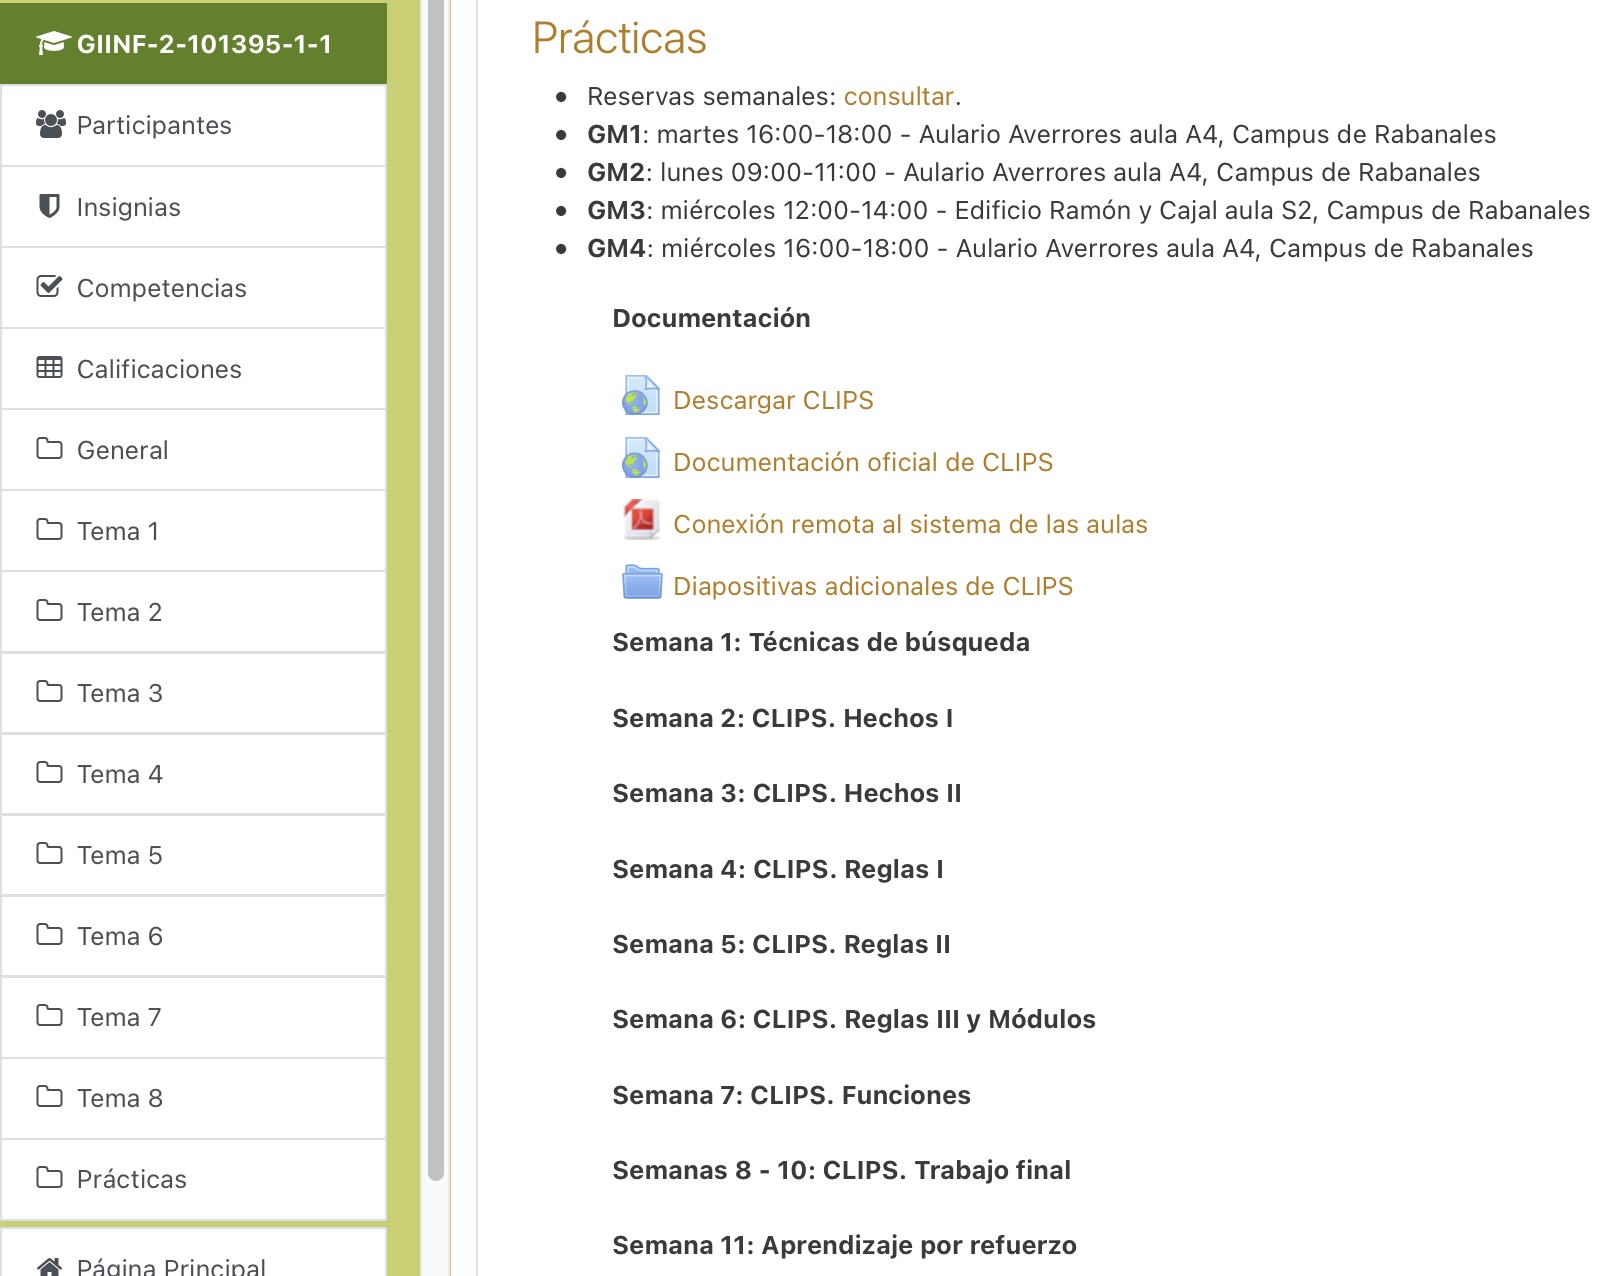
\includegraphics[width=.9\linewidth]{graphics/moodle.jpg}
	\end{minipage}
	\begin{minipage}{.38\linewidth}
		\begin{itemize}
			\item Moodle de la asignatura: \url{https://moodle.uco.es/m2223/course/view.php?id=471}
			\item Sección \textit{Prácticas} organizada por semanas.
		\end{itemize}
	\end{minipage}
\end{frame}

\begin{frame}{Evaluación de las prácticas}
    40\% de la nota final.
    Dos opciones:
    \begin{itemize}
        \item Evaluación continua – al final de la mayoría de sesiones de prácticas habrá una prueba de uno de los siguientes tipos:
        \begin{itemize}
            \item Cuestionario breve en Moodle.
            \item Desafío: pequeñas pruebas de programación para entregar a final de clase.
        \end{itemize}
        \item Examen oficial: 
        \begin{itemize}
        	\item Si la nota de la evaluación continua es inferior a 5.
        	\item Si no se va a asistir a las sesiones prácticas.
        	\item Si se quiere mejorar la nota obtenida en la evaluación continua.
        \end{itemize}
    \end{itemize}
\end{frame}

\begin{frame}{Cálculo de la nota de prácticas}
	\begin{minipage}{.55\linewidth}
    	La nota final de prácticas por evaluación continua será la media de las notas de las sesiones, valiendo todas las pruebas lo mismo.
	\end{minipage}
	\hfill
	\begin{minipage}{.38\linewidth}
    	\begin{block}{OjO}
        	La nota de la evaluación continua no se guarda si vas a examen. La nota de prácticas final será la del examen.
    	\end{block}
	\end{minipage}
\end{frame}

\againframe{firstframe}
\end{document}